
\begin{tikzpicture}
\begin{scope}
  \Text[x=-0.5,fontsize=\Large]{$\{$}
  \Vertex[size=0.5,IdAsLabel,x=0,RGB,color={231,195,138}]{07}
  \Vertex[size=0.5,IdAsLabel,x=1,RGB,color={231,195,138}]{03}
  \Vertex[size=0.5,IdAsLabel,x=2,RGB,color={231,195,138}]{05}
  \Vertex[size=0.5,IdAsLabel,x=3,RGB,color={231,195,138}]{08}
  \Text[x=3.5,fontsize=\Large, anchor=west]{$\}=x_1$}

  
  \Edge[lw=1,Direct](07)(03)
  \Edge[lw=1,Direct](03)(05)  
  \Edge[lw=1,Direct](05)(08)
\end{scope}

% \vspace{1em}

\begin{scope}[yshift=-1cm]
  \Text[x=-0.5,fontsize=\Large]{$\{$}
  \Vertex[size=0.5,IdAsLabel,x=0,RGB,color={141,203,160}]{06}
  \Vertex[size=0.5,IdAsLabel,x=1,RGB,color={141,203,160}]{05}
  \Vertex[size=0.5,IdAsLabel,x=2,RGB,color={141,203,160}]{01}
  \Vertex[size=0.5,IdAsLabel,x=3,RGB,color={141,203,160}]{08}
  \Text[x=3.5,fontsize=\Large, anchor=west]{$\}=x_2$}

  \Edge[lw=1,Direct](06)(05)
  \Edge[lw=1,Direct](05)(01)  
  \Edge[lw=1,Direct](01)(08)
\end{scope}

% \vspace{1em}

\begin{scope}[yshift=-2cm]
  \Text[x=-0.5,fontsize=\Large]{$\{$}
  \Vertex[size=0.5,IdAsLabel,x=0,RGB,color={252,98,141}]{09}
  \Vertex[size=0.5,IdAsLabel,x=1,RGB,color={252,98,141}]{10}
  \Vertex[size=0.5,IdAsLabel,x=2,RGB,color={252,98,141}]{06}
  \Vertex[size=0.5,IdAsLabel,x=3,RGB,color={252,98,141}]{02}
  \Text[x=3.5,fontsize=\Large, anchor=west]{$\}=x_3$}

  \Edge[lw=1,Direct](09)(10)
  \Edge[lw=1,Direct](10)(06)  
  \Edge[lw=1,Direct](06)(02)
\end{scope}
\end{tikzpicture}
